\newpage
\section{Verification of Lossy Channel Systems}
\label{model}
The goal of this chapter is to formalize the use of \e{small models} for the verification of lossy channel systems, as is done in \cite{parosh}. The technique is based on the use of \e{abstract interpretation} techniques, first formalized by Cousot and Cousot\cite{cousot1977}. Abstract interpretation techniques are techniques for approximating programs. Using information about the control and data flow, i.e. the semantics of a system, an overapproximation of the possible configurations of a system can be created, which is typically an infinite set of configurations. In \cite{parosh} the authors show that such an infinite set of configurations can be safely bounded to a finite set of configurations, by finding a \e{cut-off} point for the maximum size of the evaluations.


\subsection{Views}
\label{subwords}
We define a \e{view} $v= \conf{s, W}$ to be a minimal representation of a set of configurations $C_v$, such that for any $c \in C_v$, $v_E \subset c_E$ and $v_S = c_S$. Note that a view is itself a configuration, as they have the same representation, and we use the same terminology and notation for them, for example $|v|$ to denote the size. The difference is that a configuration is a single entity, whereas the view is an abstract representation of a larger set of configurations.

\paragraph{Example.} Let the view $v = \conf{(s_1, r_1), ab, cd}$, then the set $C_v$ is an infinite set, s.t. $\conf{(s_1, r_1), ab, cd} \in C_v$, $\conf{(s_1, r_1), abab, cdcd} \in C_v$ but $\conf{(s_1, r_1), ab, epsilon} NOTIN C_v$


\subsection{Abstraction function}
\label{alphagamma}
For a given parameter $k \in \mathbb{N}$, we use $C$ and $V$ to denote sets of configurations and views respectively, and $C_k$ and $V_k$ to denote the set of all configurations and views respectively of size up to $k$.

The abstraction function $\alpha_k: C\rightarrow 2^{C_k}$ maps a configuration $c$ into the powerset $V$ of views of size up to $k$, such that for each $v\in V$, $\{v_E \subseteq c_E\}$, $v_S = c_S$ and $|v_E|) \leq k$, or equivalently, $V$ is the set of views, so that $c \in (C_v \cap C_k)$ for each $v \in V$.

\paragraph{Example.} Suppose \e{c} is a configuration $\conf{s_1,r_2,ab,cd}$. The configuration is of size 2 and $\alpha_k(c)$ is the set 

\begin{ttabular}
$\{\conf{(s_1,r_2),ab,cd}$ \\
$\conf{(s_1,r_2),a,cd}$ &
$\conf{(s_1,r_2),b,cd}$ &
$\conf{(s_1,r_2),\epsilon,cd}$ \\
$\conf{(s_1,r_2),a,c}$ &
$\conf{(s_1,r_2),b,c}$ &
$\conf{(s_1,r_2),\epsilon,c}$ \\
$\conf{(s_1,r_2),a,d}$ &
$\conf{(s_1,r_2),b,d}$ &
$\conf{(s_1,r_2),\epsilon,d}$ \\
$\conf{(s_1,r_2),\epsilon,\epsilon}\}$ \\
\end{ttabular}


\subsection{Concretisation function}
The concretisation function $\gamma_k: 2^{C_k} \rightarrow 2^C$ returns, given a set of views \e{V}, the set of configurations that can be reconstructed from the views in $V$, in other words, $\gamma_k(V) = \{c \in C$ | $\alpha_k(c) \subseteq V$\}

In general $\gamma_k(V)$ is an infinite set of configurations. We define $\gamma_k^l(V)$ := $\gamma_k(V) \cap C_l$ for some $l\geq 0$. The intuitive meaning is that $\gamma_k^l(V)$ is the set of configurations of size at most $l$ for which all views of length at most $k$ are in $V$.

\subsection{Post-Image}
For a configuration $c\in C$ of a lossy transition system $LTS = (C,\rightarrow)$, we define the \e{post-image} of \e{c} denoted $\rho(c)$ = \{$c'$ | $c \rightarrow c' \in \rightarrow$\}. Intuitively, the post-image of a configuration is the configuration obtained by firing the transitions of the transition system.

For a \e{set} of configurations $V$ we define the post-image of the set $\rho(V)$ = \{$c' | c \rightarrow c' \in \rightarrow, c\in C$\}. This means that the post-image of a set $V$ of configurations is the set $\rho(V)$ containing the post-images of each configurations $c\in V$.

\subsection{Abstract Post-Image}
The \e{abstract post-image} of a set \e{V} $\subseteq$ $C_k$ is defined as $Apost_k$(\e{V}) = $\alpha_k(\rho(\gamma_k(V)))$. This means that the abstract post-image of a set $V$ is the set obtained by applying $\gamma_k$, $\rho$ and $\alpha_k$ in order to the set $V$. The procedure is illustrated in figure \ref{apost}.
\begin{figure}
\abstraction
\caption{The application order of the $\alpha$, $\rho$ and $\gamma$}
\label{apost}
\end{figure}

Note that since $V \subset Apost_k(V)$, $Apost_k$ is a monotonic function, and that the set $V$ is a powerset because the function $\alpha$ returns a powerset. This means that by the Knaster-Tarski theorem, the function $Apost_k$ has a fixpoint.
\todo[inline]{Even the infinite powerset must reach a fixpoint, right?}

\subsection{Reachability Analysis}
\label{reachcompute}
Let LTS e a lossy transition system, with initial configuration $c^0$. Then the set of reachable configurations $\mathcal{R}$ of LTS can be computed with the reccurrence, $A_0 = \{c^0\}, A_{i+1}= A_i \cup \rho(A_i)$. The finite set of configurations $\mathcal{R}_k$ with size at most $k$ can be similarly computed; $A_0$ = $\{c^0\}$, $A_{i+1} = A_i \cup (\rho(A_i) \cap C_k)$.

\subsection{Small Models}
\label{proof}
Calculating the abstract post-image of a set of views $V \subseteq C_k$ is essentiatial for the verification procedure. As $\gamma_k(V)$ typically is infinite, this cannot be done straightforwardly. It is the main result of \ref{parosh} that it suffices to consider configurations of $\gamma_k(V)$ of sizes up to $k+1$ ($\gamma_k^{k+1}$), which is a finite set of configurations for which the abstract post-image can be computed. Formally, they show that

\begin{lemma}
\label{lemma1}
For any $k\in\mathbb{N}$, and $X\subseteq C_k$, $\alpha_k(\rho(\gamma_k(X)))$ $\cup$ $X$ = $\alpha_k(\rho(\gamma_k^{k+1}(X)))$ $\cup$ $X$.
\end{lemma}
%\todo{Why is this correct? Shouldn't it be the fixpoint of the two that is equal?}

\subsubsection{Proof of lemma 1}
We want to show that the set $\gamma_k^{k+1}(X)$ of views of size at most $k+1$ is an abstract representation of the full set $gamma_k(X)$. In order to do this, we need to show that for any reachable configuration $c$ of larger size than $k+1$, all the views of $c$ of size at most $k$ are included in the set $\gamma_k(X)$ (i.e., the configuration $c$ is abstractly represented). More precisely, we want to show that for any configuration $c \in$ $\rho(\gamma_k(X))$ of size $m > k + 1$ such that there is a transition  $c' \xrightarrow{r} c$, then for each view $v' \in$ $\alpha_k(c)$, the following holds: There is a configuration $d'$ $\in$ $\gamma_k^{k+1}(X)$ of size at most $k+1$ and transition $ d' \xrightarrow{r} d$ s.t. $v \in$ $\alpha_k(d)$.

\paragraph{Transmissions}
\label{proofTransmission}
Note that by design (see section \ref{LTS}), a transmission transition changes only a single evaluation, therefore, although the set of evaluations may contain multiple evaluation, we direct our focus to a single evaluation in this section, which is explicit.

Consider a configuration $c' = \conf{s', x} \in \gamma_k(X)$ and a transition $r: c' \xrightarrow{ch_j!m} c = \conf{s,x \bullet m}$. The views $v = \conf{s', y}$ of size at most $k$ of $c$ are all have evaluations of two types:

\begin{enumerate}
\item
$y \subset x$, $|v| \leq k$. In this case, the set $\gamma_k^{k+1}$ includes all the configurations $d'$ = $\conf{s', y}$, as $d_E' \subword c_E'$. Then $d' \xrightarrow{ch_j!m} d$ yields $d = \conf{s, y\bullet m}$, for which $\conf{s, y} = v$ is a view.
\item
$y = z\bullet m$ with $z \subset x$, $|z| \leq (k-1)$. The set $\gamma_k^{k+1}$ includes all the configurations $d'$ = $\conf{s', z}$, as $d_E' \leq c_E'$. Then $d' \xrightarrow{ch_j!m} d$ yields $d = \conf{s, z\bullet m}$ which is of size at most $k$, meaning it is also a view, $d$ = $v$.
\end{enumerate}


\paragraph{Message Loss and Reception}
\label{proofreception}
The proof for reception is trivial, as removing a message from the an evaluation will not result in a word larger than the original. Thus $\alpha_k(c') \subset \alpha_k(c)$.

\paragraph{Actions}
Actions can in this context be seen as equivalent to a reception or transmission rule, reading or writing the empty symbol $\epsilon$ on some channel respectively.

\subsection{Verification Algorithm}
\label{verificationalgorithm}
As a result of lemma \ref{lemma1}, if $\gamma_k^{k+1} \cap Bad$ = $\phi$ for any \e{k} $\geq$ 1, then $\gamma_k^l(V) \cap Bad$ = $\phi$ for any larger $l \geq k$. Given a set of bad states \e{Bad}, a set of initial states \e{I} and a set of transitions, verification of a system can be done with algorithm \ref{alg1}, which was first presented in \cite{parosh}.

\begin{algorithm}
  \caption{General Verification algorithm}
  \label{alg1}
    \hspace{8pt}\textbf{for} $k := 1$ \textbf{to} $\infty$

    \hspace{16pt}\textbf{if} $\mathcal{R}_k$ $\cap$ $Bad$ $\neq$ $\emptyset$ \textbf{then return} Unsafe

    \hspace{16pt}$V := \mu X.\alpha_k(I)$ $\cup$ $Apost_k(X)$

    \hspace{16pt}\textbf{if} {$\gamma_k(V)$ $\cap$ $Bad$ = $\emptyset$} \textbf{then return} Safe
\end{algorithm}

The algorithm begins by performing a reachability analysis, as explained in \ref{reachcompute}in order to compute $\mathcal{R}_k$ and check for bad states. For any buffer size \e{k}, if a bad state is found to be reachable in $\mathcal{R}_k$, the system is unsafe and the algorithm terminates. If no such bad state was found, the algorithm continues by computing an \e{overapproximation} of configurations of size $k$, reachable through configurations of size at most $k+1$ and checking for bad configurations. This is done by computing the fixpoint of $Apost_k$. If at this point no bad configuration has been found, the system can be said to be safe and the algorithm terminates. If on the other hand a bad state was found, the system is not necessarily unsafe, as \e{V} is an overapproximation of the reachable states in $\mathcal{R}_k$. The process is then repeated with a buffer size of \e{k+1}. This process is abstractly described in the flowchart in figure \ref{flow}.

\begin{figure}
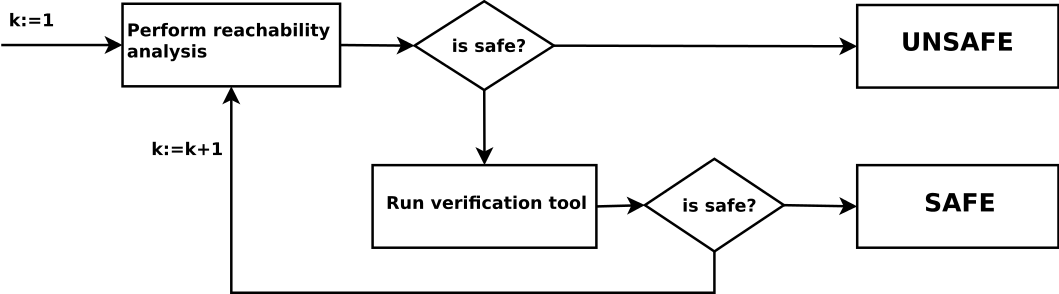
\includegraphics[width=400pt] {bilder/flowchart.png}
\caption{The general flow of the verifier.}
\label{flow}
\end{figure}
